\chapter{System Implementation}
\label{ch:implementation}

This chapter details the technical implementation of the S\textsuperscript{4}D system, covering the complete architecture from backend data processing to frontend user interface, including the dual-server approach for API services and file serving.

\section{System Architecture Overview}
\label{sec:architecture-overview}

The S\textsuperscript{4}D system employs a three-tier modular architecture with clear separation of concerns:

\begin{itemize}
    \item \textbf{Backend Processing Layer}: Python-based data processing and analysis engine
    \item \textbf{API Service Layer}: FastAPI REST API server running on port 5000
    \item \textbf{Frontend Interface Layer}: React-based web application for user interaction
    \item \textbf{File Serving Layer}: Static file server for result visualization and download
\end{itemize}

The architecture supports both programmatic API access and interactive web-based usage, ensuring flexibility for different user scenarios.

% TODO: Add figure showing system architecture overview
\begin{figure}[htbp]
    \centering
    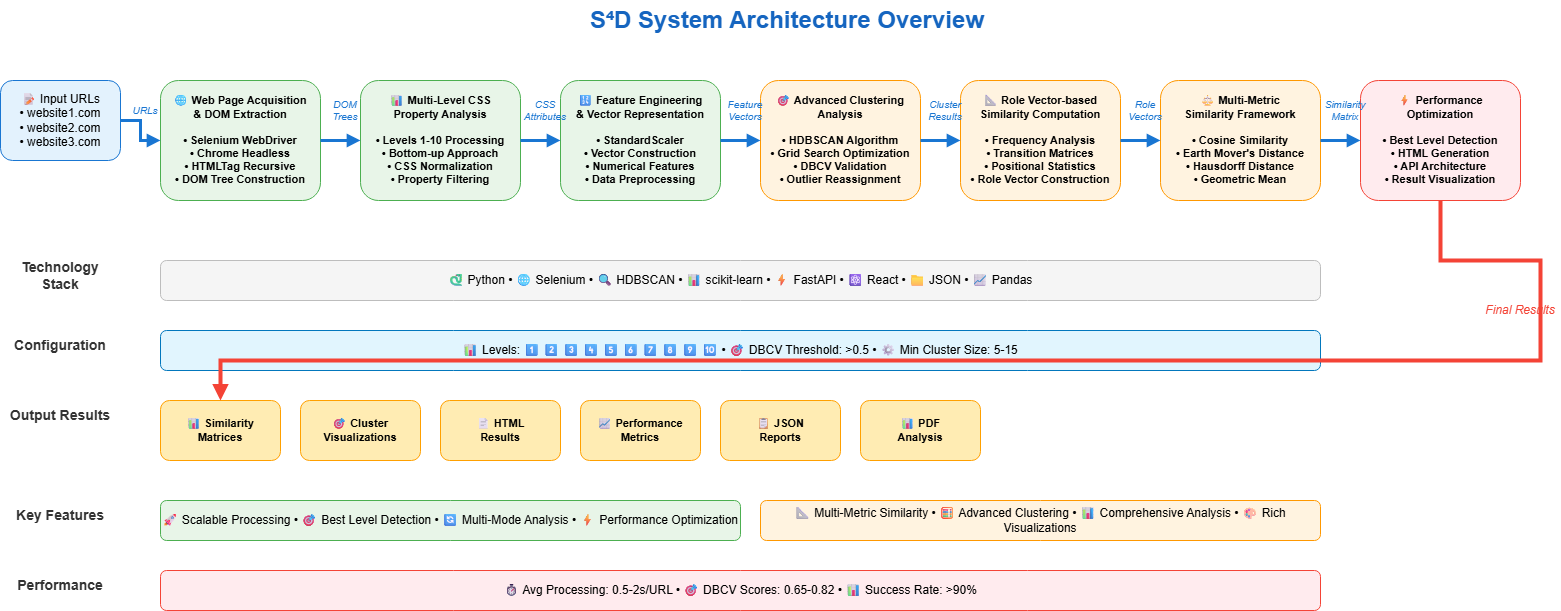
\includegraphics[width=0.9\textwidth]{figures/implementation/system_architecture_overview.png}
    \caption{S4D System Architecture Overview showing the three-tier modular design with Backend Processing Layer, API Service Layer, Frontend Interface Layer, and File Serving Layer, including communication flows and data processing pipeline.}
    \label{fig:system_architecture}
\end{figure}

\section{Backend Implementation}
\label{sec:backend-implementation}

\subsection{Core Processing Engine}
The backend implementation consists of modular Python components organized as follows:

\begin{itemize}
    \item \textbf{URL Processing Module} (\texttt{url\_scrapper.py}): Handles web page extraction and DOM parsing using Selenium WebDriver with Chrome headless browser
    \item \textbf{Similarity Computation Module} (\texttt{site\_similarity.py}): Implements multi-metric similarity algorithms including Cosine, Earth Mover's Distance (EMD), and Hausdorff distance
    \item \textbf{Clustering Module} (\texttt{clustering.py}): Provides HDBSCAN clustering with automatic parameter optimization and DBCV validation scoring
    \item \textbf{Data Collection Module} (\texttt{DataCollector.py}): Manages systematic data gathering and preprocessing for analysis
    \item \textbf{Processing Orchestration} (\texttt{process.py}): Coordinates the entire analysis pipeline from URL input to final results
\end{itemize}

\subsection{Multi-Level Analysis Implementation}
The system implements a bottom-up hierarchical analysis approach with configurable depth levels (1-10). The level system works from leaf nodes upward through the DOM tree, where each level represents the structural path length from the deepest elements:

\begin{itemize}
    \item \textbf{Level 1}: Leaf elements without children (most specific content elements)
    \item \textbf{Level 2-3}: Leaf elements with immediate structural parents (content containers)
    \item \textbf{Level 4-6}: Extended hierarchical paths capturing layout organization
    \item \textbf{Level 7-10}: Complete structural hierarchies toward root elements
\end{itemize}

This approach is implemented through the recursive DOM traversal algorithm in \texttt{url\_scrapper.py}, which builds reversed path combinations from leaf nodes upward, allowing analysis at varying levels of structural abstraction.

\section{API Implementation}
\label{sec:api-implementation}

\subsection{FastAPI Server Architecture}
The REST API is implemented using FastAPI framework, providing high-performance asynchronous request handling on localhost port 5000. The API includes four primary endpoints for core functionality:

\subsubsection{URL Processing Endpoint}
\textbf{POST /process-urls}: The primary analysis endpoint that accepts a JSON payload containing URL lists, DOM analysis levels (1-10), and processing mode configuration. The endpoint performs complete website analysis including DOM extraction, CSS property analysis, HDBSCAN clustering, and similarity computation. Returns comprehensive results including clustering configurations, similarity matrices, generated HTML visualization files, detailed timing logs, and performance metrics. Supports both unified processing (mode 0) and domain-based processing (mode 1) for scalable analysis of large URL collections.

\subsubsection{Batch Experiment Management}
\textbf{POST /experiments/run-batch}: Orchestrates large-scale experimental campaigns by accepting experiment configurations with multiple test case definitions. Each test case specifies URL sets, analysis levels, processing modes, and experimental parameters. The endpoint manages sequential execution of test cases, generates comprehensive experimental reports with statistical analysis, creates visualizations and charts using gnuplot, and stores results in organized directory structures with unique experiment identifiers. Includes progress tracking, error handling, and automatic result archiving.

\subsubsection{Results Management}
\begin{itemize}
    \item \textbf{GET /experiments/results/list}: Returns a comprehensive list of all available experiment results with detailed metadata including experiment names, execution timestamps, success rates, total test counts, processing durations, and result summary statistics. Enables users to browse historical experiments and select specific results for detailed analysis.
    \item \textbf{GET /experiments/results/\{experiment\_id\}}: Retrieves complete experimental data for a specific experiment identifier, including all test case results, generated visualizations, clustering analyses, similarity matrices, timing logs, and statistical reports. Provides access to both summary data and detailed per-test results with full clustering and similarity information.
    \item \textbf{GET /experiments/results/\{experiment\_id\}/files/\{filename\}}: Downloads specific experimental output files including gnuplot data files, generated charts, and analysis scripts. Supports direct file access for external analysis tools and result sharing.
    \item \textbf{GET /experiments/results/\{experiment\_id\}/images/\{filename\}}: Serves generated visualization images including clustering charts, similarity heatmaps, and statistical plots in multiple formats (PNG, SVG, PostScript).
\end{itemize}

\subsection{File Serving Infrastructure}
The API server also implements static file serving capabilities to provide:

\begin{itemize}
    \item \textbf{HTML Result Files}: Processed web page snapshots stored in \texttt{output\_html\_files/}
    \item \textbf{Visualization Assets}: Generated charts, graphs, and clustering visualizations
    \item \textbf{Experimental Data}: CSV files, JSON results, and statistical reports
    \item \textbf{Result Management}: Efficient storage and retrieval of analysis results
\end{itemize}

\section{Frontend Implementation}
\label{sec:frontend-implementation}

\subsection{React Application Architecture}
The frontend is implemented as a Single Page Application (SPA) using React.js, providing an intuitive interface for system interaction. The main component is \texttt{URLChipForm.js}, which manages:

\begin{itemize}
    \item \textbf{URL Input Management}: Dynamic input field with validation and URL chip visualization
    \item \textbf{Analysis Configuration}: Level selection, processing mode options, and parameter tuning
    \item \textbf{Real-time Progress Tracking}: HTTP-based progress monitoring and status updates during analysis
    \item \textbf{Results Visualization}: Interactive display of clustering results, similarity matrices, and downloadable reports
\end{itemize}

\subsection{User Interface Features}
The web interface provides comprehensive functionality including:

\begin{itemize}
    \item \textbf{Batch URL Processing}: Support for analyzing multiple URLs simultaneously
    \item \textbf{Interactive Result Exploration}: Clickable clustering visualizations and detailed similarity reports
    \item \textbf{Export Capabilities}: Download results in multiple formats (JSON, PDF, HTML)
    \item \textbf{Historical Data Access}: Browse and compare previous analysis sessions
\end{itemize}

\subsection{Integration with Backend Services}
The React frontend communicates with the backend through:

\begin{itemize}
    \item \textbf{RESTful API Calls}: Asynchronous HTTP requests to the FastAPI server
    \item \textbf{File Access Integration}: Direct links to served files for result viewing
    \item \textbf{Error Handling}: Comprehensive error management with user-friendly messages
    \item \textbf{Responsive Design}: Mobile-friendly interface adaptation
\end{itemize}

% TODO: Add figure showing React interface components and user workflow
\begin{figure}[htbp]
    \centering
    
\includegraphics[width=0.9\textwidth]{figures/interface/react_interface_overview.png}
    \caption{React Interface Overview showing the main URLChipForm component with URL input management, analysis configuration options, progress tracking, and results visualization interface for comprehensive user interaction.}
    \label{fig:react_interface}
\end{figure}

\section{Performance Optimization Implementation}
\label{sec:performance-implementation}

\subsection{Optimization Strategy}
The system implements several optimization techniques to improve performance:

\begin{itemize}
    \item \textbf{Efficient Data Structures}: Optimized data representations for large-scale processing
    \item \textbf{Memory Management}: Careful resource allocation and garbage collection
    \item \textbf{Batch Processing}: Grouped operations for improved throughput
\end{itemize}

\subsection{Scalability Considerations}
The system addresses scalability through:

\begin{itemize}
    \item \textbf{Sequential Processing}: Systematic URL processing with efficient resource utilization
    \item \textbf{Memory Management}: Efficient data structures and garbage collection
    \item \textbf{Batch Processing}: Optimized handling of large URL sets
    \item \textbf{Asynchronous Operations}: Non-blocking I/O operations for improved responsiveness
\end{itemize}

\section{Deployment and Configuration}
\label{sec:deployment-configuration}

\subsection{Development Environment Setup}
The system requires:

\begin{itemize}
    \item \textbf{Python 3.8+}: Backend processing and API server
    \item \textbf{Node.js 14+}: Frontend development and building
    \item \textbf{Chrome Browser}: Required for Selenium WebDriver operations
    \item \textbf{System Dependencies}: Various Python packages listed in requirements.txt
\end{itemize}

\subsection{Process Management and Execution}
The S\textsuperscript{4}D system utilizes \textbf{mprocs} (Multi-Process) for efficient process orchestration and management. The mprocs tool enables:

\begin{itemize}
    \item \textbf{Concurrent Service Management}: Simultaneous execution of backend API server and frontend development server
    \item \textbf{Process Monitoring}: Real-time status monitoring and log aggregation from multiple services
    \item \textbf{Simplified Deployment}: Single command execution for multi-component system startup
    \item \textbf{Development Workflow}: Streamlined development environment with automatic restart capabilities
\end{itemize}

The mprocs configuration allows developers to manage the entire S\textsuperscript{4}D ecosystem through a unified interface, significantly improving development efficiency and system reliability.

\subsection{Production Deployment Considerations}
For production deployment, the system supports:

\begin{itemize}
    \item \textbf{Docker Containerization}: Containerized deployment for consistency
    \item \textbf{Reverse Proxy Configuration}: Nginx/Apache integration for production serving
    \item \textbf{Database Integration}: Optional database backends for persistent storage
    \item \textbf{Load Balancing}: Horizontal scaling support for high-traffic scenarios
\end{itemize}

\section{Implementation Summary}
\label{sec:implementation-summary}

The S\textsuperscript{4}D implementation successfully translates the theoretical methodology into a practical, scalable system. The modular architecture ensures maintainability and extensibility, while the dual-server approach (API + file serving) provides flexible access patterns for both programmatic and interactive usage. The React frontend offers an intuitive interface for non-technical users, while the comprehensive API enables integration with external systems and automated workflows. The use of mprocs for process management ensures reliable system operation and simplified deployment.

Key implementation achievements include:
\begin{itemize}
    \item Successful integration of multiple similarity algorithms into a unified framework
    \item Efficient bottom-up multi-level analysis with configurable depth and granularity
    \item Robust error handling and graceful degradation for problematic web pages
    \item Optimized performance through efficient data structures and resource management
    \item User-friendly web interface with HTTP-based progress tracking and result visualization
    \item Comprehensive PDF export capabilities for similarity analysis reports
\end{itemize} 